%% beamer/knitr slides
%% for Statistical Modeling and Data Visualization course @ UMass
%% Nicholas Reich: nick [at] schoolph.umass.edu


\documentclass[table]{beamer}\usepackage[]{graphicx}\usepackage[]{color}
% maxwidth is the original width if it is less than linewidth
% otherwise use linewidth (to make sure the graphics do not exceed the margin)
\makeatletter
\def\maxwidth{ %
  \ifdim\Gin@nat@width>\linewidth
    \linewidth
  \else
    \Gin@nat@width
  \fi
}
\makeatother

\definecolor{fgcolor}{rgb}{0.345, 0.345, 0.345}
\newcommand{\hlnum}[1]{\textcolor[rgb]{0.686,0.059,0.569}{#1}}%
\newcommand{\hlstr}[1]{\textcolor[rgb]{0.192,0.494,0.8}{#1}}%
\newcommand{\hlcom}[1]{\textcolor[rgb]{0.678,0.584,0.686}{\textit{#1}}}%
\newcommand{\hlopt}[1]{\textcolor[rgb]{0,0,0}{#1}}%
\newcommand{\hlstd}[1]{\textcolor[rgb]{0.345,0.345,0.345}{#1}}%
\newcommand{\hlkwa}[1]{\textcolor[rgb]{0.161,0.373,0.58}{\textbf{#1}}}%
\newcommand{\hlkwb}[1]{\textcolor[rgb]{0.69,0.353,0.396}{#1}}%
\newcommand{\hlkwc}[1]{\textcolor[rgb]{0.333,0.667,0.333}{#1}}%
\newcommand{\hlkwd}[1]{\textcolor[rgb]{0.737,0.353,0.396}{\textbf{#1}}}%
\let\hlipl\hlkwb

\usepackage{framed}
\makeatletter
\newenvironment{kframe}{%
 \def\at@end@of@kframe{}%
 \ifinner\ifhmode%
  \def\at@end@of@kframe{\end{minipage}}%
  \begin{minipage}{\columnwidth}%
 \fi\fi%
 \def\FrameCommand##1{\hskip\@totalleftmargin \hskip-\fboxsep
 \colorbox{shadecolor}{##1}\hskip-\fboxsep
     % There is no \\@totalrightmargin, so:
     \hskip-\linewidth \hskip-\@totalleftmargin \hskip\columnwidth}%
 \MakeFramed {\advance\hsize-\width
   \@totalleftmargin\z@ \linewidth\hsize
   \@setminipage}}%
 {\par\unskip\endMakeFramed%
 \at@end@of@kframe}
\makeatother

\definecolor{shadecolor}{rgb}{.97, .97, .97}
\definecolor{messagecolor}{rgb}{0, 0, 0}
\definecolor{warningcolor}{rgb}{1, 0, 1}
\definecolor{errorcolor}{rgb}{1, 0, 0}
\newenvironment{knitrout}{}{} % an empty environment to be redefined in TeX

\usepackage{alltt}


%       ************************************************
%       **        LaTeX preamble to be used with all 
%	**        statsTeachR labs/handouts.
%
%	Author: Nicholas G Reich
%	Last modified: 14 January 2014
%	************************************************

% \documentclass[table]{beamer}

%	Set theme (a nice plain one)
\usetheme{Malmoe}

%	Use named colors, set main color of theme
%		to match Web site color:
\definecolor{MainColor}{RGB}{10, 74, 109}
\colorlet{MainColorMedium}{MainColor!50}
\colorlet{MainColorLight}{MainColor!20}
\usecolortheme[named=MainColor]{structure} 

%	For tables
%[dvipsnames] [table]
\usepackage{xcolor}

%% calling tabu.sty, assuming a particular directory structure
\usepackage{../../slide-includes/tabu}	% Even fancier than tabulary
\usepackage{multirow}

%	Just for the degree symbol
\usepackage{textcomp}

%	Get rid of footline (page, author, etc. on each slide)
\setbeamertemplate{footline}{}
%	Get rid of navigation buttons
\setbeamertemplate{navigation symbols}{}

%	Make footnotes not ugly
\usepackage{hanging}
\setbeamertemplate{footnote}{\raggedright\hangpara{1em}{1}\makebox[1em][l]{\insertfootnotemark}\footnotesize\insertfootnotetext\par}

%	Text style for code snippets inline in text:
\newcommand{\codeInline}[1]{\texttt{#1}}

%	Text style for emphasis stronger than \emph:
%		(Note, this doesn't toggle the way \emph does.
%			(Note, this can be done, didn't seem worth the trouble.))
\newcommand{\strong}[1]{{\bfseries{#1}}}


%        ******	Define title page	**********************
\setbeamertemplate{title page}{
	{\color{MainColor}
	% There must be a better way than this -vspace at
	%	 the top and bottom of the page to reduce the 
	%	 bottom margin, but I can't find one that works.
	\vspace{-6em}

% 	% Go to a lot of trouble to get the title in a
% 	%	nice box, since customizing a beamer block
% 	%	does not entirely work here (I don't know why)
	\newlength{\titleBoxWidth}
	\setlength{\titleBoxWidth}{\textwidth}
	\addtolength{\titleBoxWidth}{-2.0em}
	\setlength{\fboxsep}{1.0em}
	\setlength{\fboxrule}{0pt}
	\fcolorbox{MainColor!25}{MainColor!25}{
		\parbox{\titleBoxWidth}{
			\raggedright
			\LARGE\textbf{\inserttitle}
		}	% end parbox
	}	% end fcolorbox

	\vfill
	\small{Author: \insertauthor}
	\vspace{\baselineskip}

	\small{\Course}

	\small{\Instructor}
	\vspace{\baselineskip}

	%\small{\emph{This material is part of the \strong{statsTeachR} project}}

	\vspace{0.33\baselineskip}\scriptsize{\emph{\LicenseText}}


		\vspace{-15em}

	}	% end color
	\clearpage
}	% end define title page

%	The following variables are assumed by the standard preamble:
%	Global variable containing module name:
\title{Working with categorical variables as factors}
%	Global variable containing module shortname:
%		(Currently unused, may be used in future.)
\newcommand{\ModuleShortname}{introRegression}
%	Global variable containing author name:
\author{Nicholas G Reich}
%	Global variable containing text of license terms:
\newcommand{\LicenseText}{Made available under the Creative Commons Attribution-ShareAlike 3.0 Unported License: http://creativecommons.org/licenses/by-sa/3.0/deed.en\textunderscore US }
%	Instructor: optional, can leave blank.
%		Recommended format: {Instructor: Jane Doe}
\newcommand{\Instructor}{}
%	Course: optional, can leave blank.
%		Recommended format: {Course: Biostatistics 101}
\newcommand{\Course}{}


\input{../../slide-includes/shortcuts}

\hypersetup{colorlinks,linkcolor=,urlcolor=MainColor}


%	******	Document body begins here	**********************
\IfFileExists{upquote.sty}{\usepackage{upquote}}{}
\begin{document}

%	Title page
\begin{frame}[plain]
	\titlepage
\end{frame}

%	******	Everything through the above line must be placed at
%		the top of any TeX file using the statsTeachR standard
%		beamer preamble.




%%%%%%%%%%%%%%%%%%%%%%%%%%%%%%%%%%%%%%%%%%

\begin{frame}{Different kinds of variables}
\begin{block}{Give some examples of each}

\bi
    \item Continuous: variables taking any real number value in a range
    \vspace{4em}
    \item Discrete: variables taking an integer value
    \vspace{4em}
    \item Categorical: variables taking one of a fixed set of values
\ei

\end{block}

\end{frame}


%%%%%%%%%%%%%%%%%%%%%%%%%%%%%%%%%%%%%%%%%%

\begin{frame}[fragile]{Categorical variables in R often start as strings}

By default, characters are read in as characters, not as factors, although you can force factors.
A factor is a special type of R data type that can be used to represent a categorical variable with a fixed number of responses.

\begin{knitrout}\tiny
\definecolor{shadecolor}{rgb}{0.969, 0.969, 0.969}\color{fgcolor}\begin{kframe}
\begin{alltt}
\hlkwd{library}\hlstd{(tidyverse)}
\hlstd{co2} \hlkwb{<-} \hlkwd{read_csv}\hlstd{(}\hlstr{"../../data/co2emissions.csv"}\hlstd{)}
\hlkwd{head}\hlstd{(co2)}
\end{alltt}
\begin{verbatim}
## # A tibble: 6 x 3
##    Year   CO2 Type        
##   <dbl> <dbl> <chr>       
## 1  1980  81.2 Rural Diesel
## 2  1981  89.9 Rural Diesel
## 3  1982  89.9 Rural Diesel
## 4  1983  95.7 Rural Diesel
## 5  1984  95.7 Rural Diesel
## 6  1985  95.7 Rural Diesel
\end{verbatim}
\end{kframe}
\end{knitrout}


\end{frame}


%%%%%%%%%%%%%%%%%%%%%%%%%%%%%%%%%%%%%%%%%%

\begin{frame}[fragile]{Tidy aggregation and summary by category}

We can use {\tt group\_by()} and {\tt summarize()} to aggregate and compute summaries by categories. (You will be asked to do this in a future coding challenge.)

For example, here we compute the average CO2 emissions across all years, for each type of vehicle.

\begin{knitrout}\tiny
\definecolor{shadecolor}{rgb}{0.969, 0.969, 0.969}\color{fgcolor}\begin{kframe}
\begin{alltt}
\hlstd{co2} \hlopt
  \hlkwd{group_by}\hlstd{(Type)} \hlopt
  \hlkwd{summarize}\hlstd{(}\hlkwc{mean_emissions} \hlstd{=} \hlkwd{mean}\hlstd{(CO2))}
\end{alltt}
\begin{verbatim}
## # A tibble: 4 x 2
##   Type           mean_emissions
##   <chr>                   <dbl>
## 1 Rural Diesel             146.
## 2 Rural Gasoline           390.
## 3 Urban Diesel             127.
## 4 Urban Gasoline           669.
\end{verbatim}
\end{kframe}
\end{knitrout}

\end{frame}


%%%%%%%%%%%%%%%%%%%%%%%%%%%%%%%%%%%%%%%%%%

\begin{frame}[fragile]{Tidy aggregation and summary by category}

You can compute multiple summaries at once.

\begin{knitrout}\tiny
\definecolor{shadecolor}{rgb}{0.969, 0.969, 0.969}\color{fgcolor}\begin{kframe}
\begin{alltt}
\hlstd{co2} \hlopt
  \hlkwd{group_by}\hlstd{(Type)} \hlopt
  \hlkwd{summarize}\hlstd{(}
    \hlkwc{mean_emissions} \hlstd{=} \hlkwd{mean}\hlstd{(CO2),}
    \hlkwc{max_emissions} \hlstd{=} \hlkwd{max}\hlstd{(CO2),}
    \hlkwc{min_emissions} \hlstd{=} \hlkwd{min}\hlstd{(CO2))}
\end{alltt}
\begin{verbatim}
## # A tibble: 4 x 4
##   Type           mean_emissions max_emissions min_emissions
##   <chr>                   <dbl>         <dbl>         <dbl>
## 1 Rural Diesel             146.          209.          81.2
## 2 Rural Gasoline           390.          446.         348. 
## 3 Urban Diesel             127.          203.          46.4
## 4 Urban Gasoline           669.          820.         516.
\end{verbatim}
\end{kframe}
\end{knitrout}

\end{frame}

%%%%%%%%%%%%%%%%%%%%%%%%%%%%%%%%%%%%%%%%%%

\begin{frame}[fragile]{Using categorical variables for aesthetics}

Note that R translates the character variable into a factor for you without you doing anything.

\begin{knitrout}\tiny
\definecolor{shadecolor}{rgb}{0.969, 0.969, 0.969}\color{fgcolor}\begin{kframe}
\begin{alltt}
\hlkwd{ggplot}\hlstd{(co2,} \hlkwd{aes}\hlstd{(}\hlkwc{x} \hlstd{= Year,} \hlkwc{y} \hlstd{= CO2,} \hlkwc{shape} \hlstd{= Type,} \hlkwc{fill} \hlstd{= Type))}\hlopt{+}
  \hlkwd{geom_point}\hlstd{()}
\end{alltt}
\end{kframe}

{\centering 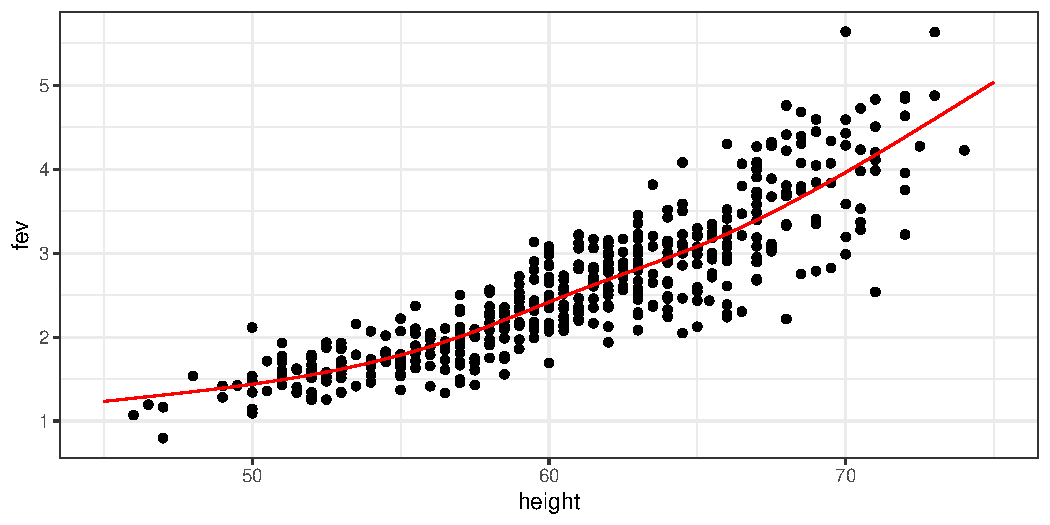
\includegraphics[width=\maxwidth]{figure/beamer-unnamed-chunk-4-1} 

}


\end{knitrout}

\end{frame}

%%%%%%%%%%%%%%%%%%%%%%%%%%%%%%%%%%%%%%%%%%

\begin{frame}[fragile]{Using factors for aesthetics}

Note that you can get the same result by explicitly calling Type a {\tt factor}.

\begin{knitrout}\tiny
\definecolor{shadecolor}{rgb}{0.969, 0.969, 0.969}\color{fgcolor}\begin{kframe}
\begin{alltt}
\hlkwd{ggplot}\hlstd{(co2,} \hlkwd{aes}\hlstd{(}\hlkwc{x} \hlstd{= Year,} \hlkwc{y} \hlstd{= CO2,} \hlkwc{shape} \hlstd{=} \hlkwd{factor}\hlstd{(Type),} \hlkwc{fill} \hlstd{=} \hlkwd{factor}\hlstd{(Type)))}\hlopt{+}
  \hlkwd{geom_point}\hlstd{()}
\end{alltt}
\end{kframe}

{\centering 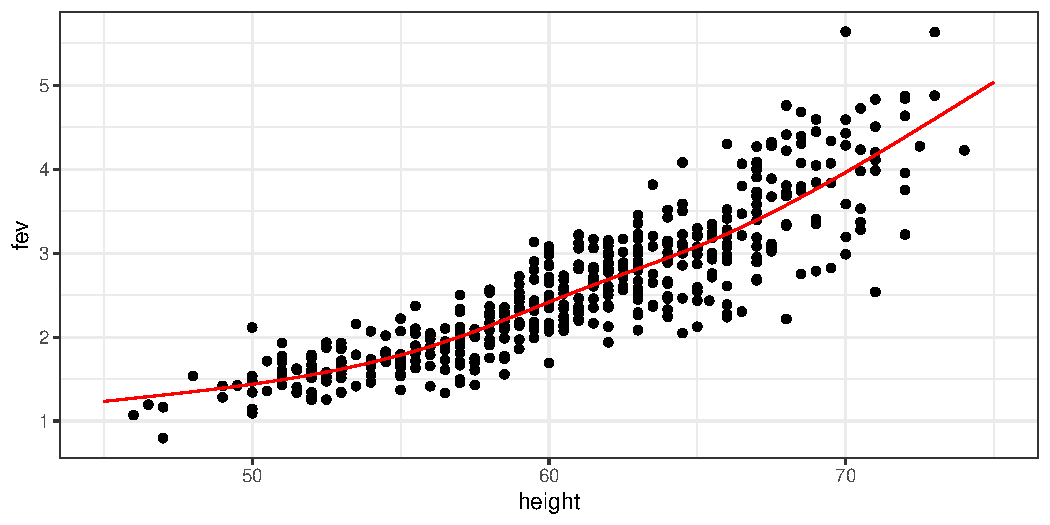
\includegraphics[width=\maxwidth]{figure/beamer-unnamed-chunk-5-1} 

}


\end{knitrout}

\end{frame}

%%%%%%%%%%%%%%%%%%%%%%%%%%%%%%%%%%%%%%%%%%

\begin{frame}[fragile]{Using factors for aesthetics}

And with just a few small tweaks, we can customize

\begin{knitrout}\tiny
\definecolor{shadecolor}{rgb}{0.969, 0.969, 0.969}\color{fgcolor}\begin{kframe}
\begin{alltt}
\hlstd{levels} \hlkwb{<-} \hlkwd{c}\hlstd{(}\hlstr{"Urban Gasoline"}\hlstd{,} \hlstr{"Rural Gasoline"}\hlstd{,} \hlstr{"Urban Diesel"}\hlstd{,} \hlstr{"Rural Diesel"}\hlstd{)}
\hlkwd{ggplot}\hlstd{(co2,} \hlkwd{aes}\hlstd{(}\hlkwc{x} \hlstd{= Year,} \hlkwc{y} \hlstd{= CO2,} \hlkwc{shape} \hlstd{= Type,} \hlkwc{fill} \hlstd{= Type))} \hlopt{+}
  \hlkwd{geom_point}\hlstd{()} \hlopt{+}
  \hlkwd{scale_shape_manual}\hlstd{(}\hlkwc{breaks}\hlstd{=levels,} \hlkwc{values}\hlstd{=}\hlkwd{c}\hlstd{(}\hlnum{24}\hlstd{,} \hlnum{21}\hlstd{,} \hlnum{24}\hlstd{,} \hlnum{21}\hlstd{))} \hlopt{+}
  \hlkwd{scale_fill_manual}\hlstd{(}\hlkwc{breaks} \hlstd{= levels,}
                    \hlkwc{values}\hlstd{=}\hlkwd{c}\hlstd{(}\hlstr{"blue4"}\hlstd{,} \hlstr{"dodgerblue"}\hlstd{,} \hlstr{"orangered"}\hlstd{,} \hlstr{"orange"}\hlstd{))} \hlopt{+}
  \hlkwd{ylab}\hlstd{(}\hlkwd{expression}\hlstd{(CO[}\hlnum{2}\hlstd{]}\hlopt{*}\hlstr{" (Mt)"}\hlstd{))}
\end{alltt}
\end{kframe}

{\centering 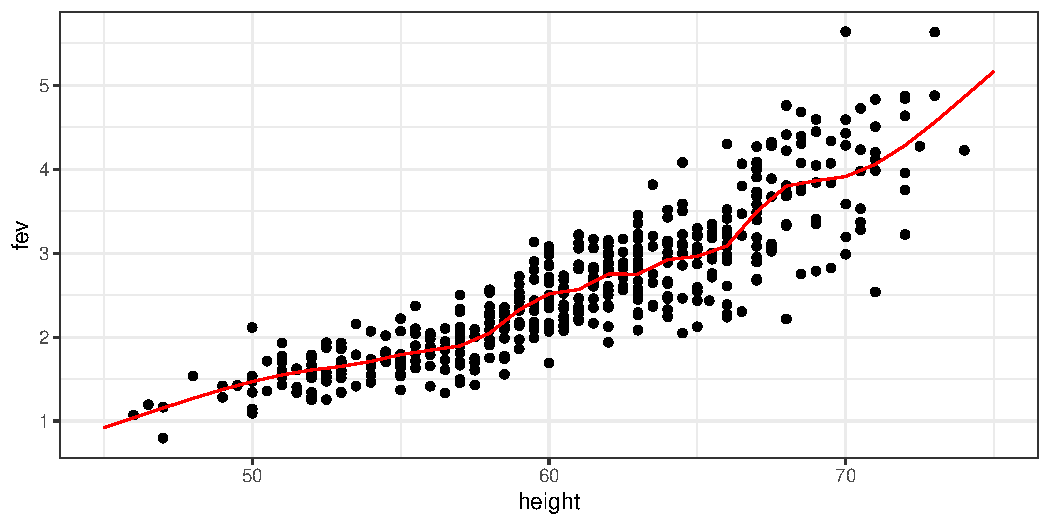
\includegraphics[width=\maxwidth]{figure/beamer-unnamed-chunk-6-1} 

}


\end{knitrout}

\end{frame}

%%%%%%%%%%%%%%%%%%%%%%%%%%%%%%%%%%%%%%%%%%

\begin{frame}[fragile]{Using factors for faceting}

Factors (or any variable with a small number of distinct values) can be used to create facets as well.

\begin{knitrout}\tiny
\definecolor{shadecolor}{rgb}{0.969, 0.969, 0.969}\color{fgcolor}\begin{kframe}
\begin{alltt}
\hlkwd{ggplot}\hlstd{(co2,} \hlkwd{aes}\hlstd{(}\hlkwc{x} \hlstd{= Year,} \hlkwc{y} \hlstd{= CO2))} \hlopt{+}
  \hlkwd{geom_point}\hlstd{()} \hlopt{+}
  \hlkwd{facet_wrap}\hlstd{(}\hlopt{~}\hlstd{Type)}
\end{alltt}
\end{kframe}

{\centering \includegraphics[width=\maxwidth]{figure/beamer-unnamed-chunk-7-1} 

}


\end{knitrout}

\end{frame}


%%%%%%%%%%%%%%%%%%%%%%%%%%%%%%%%%%%%%%%%%%

\begin{frame}[fragile]{Advanced use of factors: ordering}

Turning categorical variables into ordered factors might help you show more data.

\begin{knitrout}\tiny
\definecolor{shadecolor}{rgb}{0.969, 0.969, 0.969}\color{fgcolor}\begin{kframe}
\begin{alltt}
\hlstd{gapminder} \hlkwb{<-} \hlkwd{read_csv}\hlstd{(}\hlstr{"../../data/gapminder.csv"}\hlstd{)} \hlopt
    \hlkwd{filter}\hlstd{(continent} \hlopt \hlkwd{c}\hlstd{(}\hlstr{"Africa"}\hlstd{,} \hlstr{"Oceania"}\hlstd{))}
\hlkwd{ggplot}\hlstd{(gapminder,} \hlkwd{aes}\hlstd{(}\hlkwc{x}\hlstd{=year,} \hlkwc{y}\hlstd{=country,} \hlkwc{fill}\hlstd{=lifeExp))} \hlopt{+}
    \hlkwd{geom_tile}\hlstd{()}
\end{alltt}
\end{kframe}

{\centering \includegraphics[width=\maxwidth]{figure/beamer-unnamed-chunk-8-1} 

}


\end{knitrout}

\end{frame}


%%%%%%%%%%%%%%%%%%%%%%%%%%%%%%%%%%%%%%%%%%

\begin{frame}[fragile]{Advanced use of factors: ordering}

If ``order matters'' for your categorical variable, then turning it into an ordered factor might be useful.

\begin{knitrout}\tiny
\definecolor{shadecolor}{rgb}{0.969, 0.969, 0.969}\color{fgcolor}\begin{kframe}
\begin{alltt}
\hlcom{## this redefines country based on average GDP}
\hlstd{gapminder} \hlkwb{<-} \hlkwd{mutate}\hlstd{(gapminder,} \hlkwc{country} \hlstd{=} \hlkwd{reorder}\hlstd{(country, gdpPercap,} \hlkwc{FUN}\hlstd{=mean))}

\hlkwd{ggplot}\hlstd{(gapminder,} \hlkwd{aes}\hlstd{(}\hlkwc{x}\hlstd{=year,} \hlkwc{y}\hlstd{=country,} \hlkwc{fill}\hlstd{=lifeExp))} \hlopt{+}
    \hlkwd{geom_tile}\hlstd{()}
\end{alltt}
\end{kframe}

{\centering \includegraphics[width=\maxwidth]{figure/beamer-unnamed-chunk-9-1} 

}


\end{knitrout}

\end{frame}

%%%%%%%%%%%%%%%%%%%%%%%%%%%%%%%%%%%%%%%%%%

\begin{frame}[fragile]{Advanced use of factors: ordering}

Here we order based on the maximum GDP rather than the mean.

\begin{knitrout}\tiny
\definecolor{shadecolor}{rgb}{0.969, 0.969, 0.969}\color{fgcolor}\begin{kframe}
\begin{alltt}
\hlcom{## this redefines country based on max GDP}
\hlstd{gapminder} \hlkwb{<-} \hlkwd{mutate}\hlstd{(gapminder,} \hlkwc{country} \hlstd{=} \hlkwd{reorder}\hlstd{(country, gdpPercap,} \hlkwc{FUN}\hlstd{=max))}

\hlkwd{ggplot}\hlstd{(gapminder,} \hlkwd{aes}\hlstd{(}\hlkwc{x}\hlstd{=year,} \hlkwc{y}\hlstd{=country,} \hlkwc{fill}\hlstd{=lifeExp))} \hlopt{+}
    \hlkwd{geom_tile}\hlstd{()}
\end{alltt}
\end{kframe}

{\centering \includegraphics[width=\maxwidth]{figure/beamer-unnamed-chunk-10-1} 

}


\end{knitrout}

\end{frame}

%%%%%%%%%%%%%%%%%%%%%%%%%%%%%%%%%%%%%%%%%%

\begin{frame}[fragile]{Trying out different color scales}

Using color scales from ColorBrewer: \href{https://colorbrewer2.org/}{colorbrewer2.org}.

\begin{knitrout}\tiny
\definecolor{shadecolor}{rgb}{0.969, 0.969, 0.969}\color{fgcolor}\begin{kframe}
\begin{alltt}
\hlkwd{ggplot}\hlstd{(gapminder,} \hlkwd{aes}\hlstd{(}\hlkwc{x}\hlstd{=year,} \hlkwc{y}\hlstd{=country,} \hlkwc{fill}\hlstd{=lifeExp))} \hlopt{+}
    \hlkwd{geom_tile}\hlstd{()} \hlopt{+}
    \hlkwd{scale_fill_gradient}\hlstd{(}\hlkwc{low}\hlstd{=}\hlstr{"#fff7fb"}\hlstd{,} \hlkwc{high}\hlstd{=}\hlstr{"#034e7b"}\hlstd{)}
\end{alltt}
\end{kframe}

{\centering \includegraphics[width=\maxwidth]{figure/beamer-unnamed-chunk-11-1} 

}


\end{knitrout}

\end{frame}

%%%%%%%%%%%%%%%%%%%%%%%%%%%%%%%%%%%%%%%%%%

\begin{frame}[fragile]{Trying out different color scales}

And from the {\tt viridis} package.

\begin{knitrout}\tiny
\definecolor{shadecolor}{rgb}{0.969, 0.969, 0.969}\color{fgcolor}\begin{kframe}
\begin{alltt}
\hlkwd{library}\hlstd{(viridis)}
\hlkwd{ggplot}\hlstd{(gapminder,} \hlkwd{aes}\hlstd{(}\hlkwc{x}\hlstd{=year,} \hlkwc{y}\hlstd{=country,} \hlkwc{fill}\hlstd{=lifeExp))} \hlopt{+}
    \hlkwd{geom_tile}\hlstd{()} \hlopt{+}
    \hlkwd{scale_fill_viridis}\hlstd{()}
\end{alltt}
\end{kframe}

{\centering \includegraphics[width=\maxwidth]{figure/beamer-unnamed-chunk-12-1} 

}


\end{knitrout}

\end{frame}

%%%%%%%%%%%%%%%%%%%%%%%%%%%%%%%%%%%%%%%%%%

\begin{frame}[fragile]{Trying out different color scales}

\begin{knitrout}\tiny
\definecolor{shadecolor}{rgb}{0.969, 0.969, 0.969}\color{fgcolor}\begin{kframe}
\begin{alltt}
\hlkwd{ggplot}\hlstd{(gapminder,} \hlkwd{aes}\hlstd{(}\hlkwc{x}\hlstd{=year,} \hlkwc{y}\hlstd{=country,} \hlkwc{fill}\hlstd{=lifeExp))} \hlopt{+}
    \hlkwd{geom_tile}\hlstd{()} \hlopt{+}
    \hlkwd{scale_fill_viridis}\hlstd{(}\hlkwc{direction}\hlstd{=}\hlopt{-}\hlnum{1}\hlstd{)}
\end{alltt}
\end{kframe}

{\centering \includegraphics[width=\maxwidth]{figure/beamer-unnamed-chunk-13-1} 

}


\end{knitrout}

\end{frame}

%%%%%%%%%%%%%%%%%%%%%%%%%%%%%%%%%%%%%%%%%%

\begin{frame}[fragile]{Breakout rooms}

Work with your group on the following:

\begin{itemize}
  \item as a group, finish the note-catcher for last week, on recreating the improving the C02 emissions figure.
  \item start to look for an article for Lab 2 (see assignment on Moodle). You must complete this assignment on your own, but it's recommended to find an article that you can work in parallel with 1-2 other people on.
\end{itemize}

\end{frame}


%%%%%%%%%%%%%%%%%%%%%%%%%%%%%%%%%%%%%%%%%%





%%%%%%%%%%%%%%%%%%%%%%%%%%%%%%%%%%%%%%%%%%



\end{document}
